\chapter{La storia del software libero}


\section{Gli albori}

1950 - 1960, la cultura hacker nasce ai laboratori del \textbf{MIT}. Nel 58/59 nascono i primi corsi di \textbf{intelligenza artificiale} (di fatto era informatica). Vi era un rapporto \textit{giocoso} tra il gruppo di ricerca e i ragazzi, un rapporto che funzionava molto bene. Il primo gruppo hacker nasce dal sottogruppo del Tech Model Railroad Club un club per appassionati di modellismo, lo S\&P che si occupava della parte elettronica. All'inizio non era una vera e propria comunità hacker ma c'era solamente un gruppo che frequentava i corsi. L'accesso ai PC all'epoca era molto riservato (ai docenti, al personale). Questo gruppo aveva trovato una sala (407) con delle macchine perforatrici (per programmare le schede perforate). 

Il rapporto cambierà con l'evoluzione delle tecnologie, con l'accesso più libero alle nuove macchine (TX0). Con il cambiamento delle tecnologie cambia anche la gestione (si poteva accedere liberamente alle macchine), si cominciò a formare un gruppo di persone che \textit{bazzicavano} sulle macchine. Si formò così una comunità con idee e un'etica in comune. 

Con il PDP (computer) le cose cambiarono ulteriormente. I PDP era pensato non per il \textit{best-processing} ma per una computazione interattiva (aveva un monitor ...), costava inoltre molto meno ed era quindi più accessibile. A quel punto diventava possibile utilizzare le macchine a costo zero.

\section{Etica hacker}

L'etica che si sviluppò all'interno della comunità si basava sui seguenti 4 punti:

\begin{enumerate}

\item \textbf{Libero accesso all'informazione}, bisogna poter metterci le mani, e questo non era all'epoca garantito a tutti;
\item \textbf{Decentralizzazione}, potere che si sposta dal centro, occorre avere un sistema aperto e privo di ostacoli per favorire il libero accesso all'informazione, senza rallentamenti burocratici;
\item Gli hacker dovrebbero essere \textbf{giudicati solo per il loro valore};
\item Il software come \textbf{espressione artistica}, va oltre quello che è la pura utilità, va a fare qualcosa che è divertente e bello (creazione di giochi). Doveva essere un piacere che andasse agli altri;

\end{enumerate}

\section{Incompatible Time Sharing}

In questo momento c'è una libera condivisione del codice, non esiste software protetto da copyright visto che non c'era interesse nel proteggerlo. 
Il software era un'appendice dell'hardware. Le macchine erano in continua evoluzione e modifica. 
L'avere un accesso a come il software funzionava era vitale per gli sviluppatori. 
Dato che il tempo macchina era oneroso, bisognava sfruttarlo al meglio e quindi era importante la condivisione del lavoro tra gli sviluppatori.

Per soddisfare queste necessità il movimento hacker del MIT ha realizzato \textbf{Incompatible Time Sharing} (ITS), un sistema operativo per il PDP-10\footnote{Mainframe fabbricato dalla Digital Equipment Corporation progettato per funzionare in time-sharing.} che funzionava in time-sharing.

ITS doveva essere anche un'alternativa a Multics, un altro sistema operativo il cui sviluppo veniva supervisionato dal progetto MAC\footnote{Un gruppo di ricerca del MIT finanziato anche dalla DARPA,} e che andava contro i principi dell'etica hacker. In particolare gli standard di sicurezza del progetto Multics erano troppo elevati ed impedivano il libero accesso all'informazione.

Una delle caratteristiche principali di ITS era quella di avere l'accesso condiviso ai file tra i computer, questo grazie anche al collegamento con ARPAnet. 
L'accesso al sistema era libero, senza password e ogni utente aveva i propri file personali accessibili da tutti. 
Era disegnato per la cooperazione tra gli hacker ed assumeva una grossa fiducia negli utenti.
Il nome ITS è una parodia sul nome \textbf{C}ompatible \textbf{T}ime \textbf{S}haring \textbf{S}ystem, un'altro sistema operativo precedentemente utilizzato dal MIT.

Riassumendo le caratteristiche di ITS:

\begin{itemize}
	\item Presenza di utenti multipli, ma forniva anche la possibilità di eseguire più programmi contemporaneamente.
	\item Mancanza di password e permessi.
	\item Possibilità di avere dei file personali, ma comunque consultabili da tutti.
	\item Possibilità di accedere da terminali diversi
	\item Funzionamento sia in time-sharing, durante il giorno, che in single-mode, durante la notte, in modo da poter eseguire anche programmi computazionalmente complessi.
\end{itemize}

Tuttavia, nel '68 il laboratorio degli hacker viene isolato, scegliendo di utilizzare TENEX come sistema operativo per il PDP-10 al posto di ITS, segnando così l'inizio della crisi del periodo degli hacker.

\section{L'ultimo degli Hacker - Richard Stallman}

Analizziamo la fase di decadenza degli hacker, qui entra in gioco Richard Stallman.

\subsection{Prime esperienze}

Richard Stallman nasce a New York nel 1953 dove si forma dal punto di vista informatico, diventa un esperto di Assembler, di sistemi operativi e di editor di testo. Inizia con le prime esperienze nel centro scientifico di Manhattan, poi lo assumono e inizia a sviluppare programmi in Fortran per il calcolo numerico. Nel 1971 entra ad Harvard e si laurea in Fisica. Scopre in segreto un'affinità con la cultura hacker sviluppatasi al MIT. Venne notato da Russ Noftsker e in seguito assunto al MIT come programmatore di sistemi. Viene preso sotto l'ala protettiva di Richard Greenblatt e Bill Gosper, che gli fanno da mentore.

\begin{figure}[htbp]
	\centering
	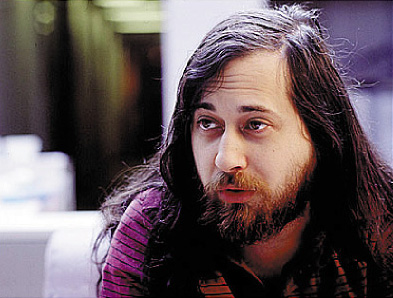
\includegraphics[width=50mm]{images/stallman.jpg}
	\caption{Richard Stallmann da giovane}
\end{figure}

\subsection{Emacs}

Una delle prime cose che Stallman fece fu la creazione di Emacs. 
Inizialmente esso era pensato come un insieme di macro per TECO, utilizzato da tutti, che era una sorta di linguaggio per scrivere e non era assolutamente real-time. 
Creò dunque una sorta di editor dentro TECO.  Guy Steele ebbe in seguito l'idea di fare un po' di ordine tra le macro (che erano diventate tantissime). 
Quest'opera fu continuata da Stallman, in modo da avere un insieme più omogeneo. Questo disordine non sarebbe dovuto replicarsi in futuro, bisognava evitare che ciascuno costruisse il proprio insieme di macro. Stallman voleva fare qualcosa di ``sociale'', voleva andare un po' oltre e impedire ulteriori disordini. Quindi si imposero delle restrizioni sulle modifiche delle macro. Questa condizione creò una sorta di comunità in cui i programmatori condividevano gli sforzi di programmazione ed evitavano la dispersione del lavoro. Questo fu il primo gruppo concreto di condivisione del software e il primo mattone della nascita della GPL. Emacs è nato in questo modo, ma poi è stato ritradotto varie volte.

\begin{figure}[htbp]
	\centering
	
\includegraphics[width=20mm]{images/emacs.png}
	\caption{Il logo di emacs}
\end{figure}

\section{La crisi del movimento hacker del MIT}

\subsection{Le prime incursioni}

Si iniziarono a vedere e prime debolezze quando il dipartimento di difesa obbligò gli hackers a programmare sui sistemi del dipartimento di \textit{computer science} del MIT in cui c'era mancanza di accesso libero all'informazione. 

Gli hacker arrivarono quindi al punto di fare una sorta di ``sciopero'' nei confronto del laboratorio, bloccarono anche l'accesso alle successive versioni di Emacs. 

Negli anni '70-'80 si creò poi una frammentazione all'interno della cultura hacker, questo perché molti hackers cominciarono a migrare, andando a lavorare per altre società.

Inoltre, iniziarono a comparire i primi programmi coperti da copyright anche all'interno del MIT.

\subsection{La Lisp machine e il collasso}

Richard Greenblatt, un programmatore del MIT, era un'autorità nel settore. 
Aveva iniziato a giocare con le LISP machine (LISP era un linguaggio ad alto livello) e aveva avuto l'idea di creare una macchina che eseguisse LISP in modo più efficiente e sicuro. 
Creò una sorta di controllo all'interno di LISP per la gestione delle risorse, aveva modificato la struttura dell'hardware in modo che LISP venisse utilizzato più velocemente. 
Questo fu un grosso passo avanti, perché programmare in LISP era molto più comodo che programmare in Assembler. 
Alla lunga riuscì ad ottenere lo stanziamento di fondi per 6 macchine. Si arrivò a produrne 32. 

Anche per gli hacker era un mondo nuovo, perché cambiava la visione classica (un solo computer disponibile), ora ogni persona aveva la propria macchina. Pensò dunque di collegare queste 32 macchine per favorire la condivisione. 
Il progetto è cresciuto a un punto tale che si trasformò in un azienda per la produzione di Lisp machine, che in un certo senso era un'estensione del MIT. 

La visione di Greenblatt era quella di un'azienda \textit{``hacker friendly''}, da mantenere senza coinvolgere investitori esterni, ma reinvestendo i soldi anticipati dai clienti. 
Russel Noftsker, che era parte del progetto, non condivideva molto l'idea e la sua visione era incompatibile con quella di Greenblatt, infatti pensava che con questa politica l'azienda non sarebbe stata in grado di funzionare e voleva adottare una struttura aziendale più classica, dando del poter anche agli investitori esterni.

Nel 1979 si arriva al punto in cui il conflitto esplode (Greenblatt aveva dalla sua un caratteraccio, non teneva conto delle persone). Da un lato non si poteva ``far fuori Greenblatt'', ma dall'altro non c'erano molte persone che volessero continuare con la sua visione (Greenblatt voleva avere l'ultima parola), quindi in sostanza non esisteva un team. 
 
 Vennero quindi fondate due aziende, la \textbf{Lisp Machine, Inc} (LMI) di Greenblatt e la \textbf{Symbolics Inc} di Noftsker.
 
 \subsection{Lo svuotamento del MIT}
 
LMI e Symbolics attingono pesantemente dal MIT, dividendo così la comunità. 
Nel 1982 Symbolics rende le proprie modifiche al sistema operativo delle Lisp machines proprietario. A questo punto c'è un crollo della comunità, era già molto debole, erano rimasti pochi hackers ma c'era comunque un sistema complesso che andava mantenuto. 
 
Quindi a un certo punto PDP divenne obsoleto e la comunità si ritrovò di fronte a un problema, bisognava creare una nuova macchina, era necessario prendere tutto il software delle macchine correnti e riscriverlo, e gli hackers non erano abbastanza numerosi. 
 
Alla fine si decise di comprare il sistema operativo proprietario di Digital e a partire da esso si creò \textbf{Twenex}, con caratteristiche molto diverse da un sistema standard (sicurezza costruita nel sistema). 
Il gruppo \textit{wheel} era un gruppo i cui programmatori erano gli unici che potevano divenire amministratori e apportare modifiche alla macchina. In seguito ci fu la nascita di GNU.

\
\section{Il progetto GNU}

\subsection{In principio c'erano UNIX e BSD}

Durante il periodo hacker del MIT, il progetto MAC, finanziato dalla DARPA, stava sviluppando Multics, un sistema operativo modulare, facile da estendere e da riconfigurare.
Questo sistema però è risultato troppo complesso e ciò ha portato al fallimento commerciale del progetto.

All'interno del progetto Multics c'era anche AT\&T, che nel 1969 decide di abbandonarlo. Tuttavia, Dennis Richie e Ken Thompson continuano la a sviluppare le idee alla base di Multics e sviluppano una versione più leggera del sistema operativo, così nel 1972 nasce UNIX.

In quel periodo AT\&T aveva il monopolio telefonico e quindi non poteva commercializzare software, pertanto UNIX è stato distribuito liberamente.

Tra le varie versioni modificate di UNIX c'è BSD, la versione sviluppata da due studenti della Berkley, Chuck Haley e Bill Joy, che comprendeva dei miglioramenti al kernel, un editor di testo e un compilatore Pascal. 

La prima versione di BSD viene rilasciata nel 1978  e nel 1980 la DARPA stanzia dei fondi per portare avanti lo sviluppo di BSD, il quale doveva essere utilizzato per costruire ARPANET. 
Nasce così il Computer Systems Reserach Group, guidato da Bill Joy e nel 1980 viene rilasciato 4BSD.

Successivamente vennero rilasciate altre versioni, come la 4.1aBSD che conteneva la bozza del protocollo TCP/IP e la 4.3BSD che implementò la prima versione di TCP/IP (1986), protocollo che verrà poi scelto dalla DARPA come standard per le comunicazioni di rete. 

Nel 1979 AT\&T annuncia di voler commercializzare UNIX e nel 1983, dopo essere stata scorporata, UNIX diventa commerciale e viene distribuito con licenze molto costose. Si iniziò quindi a staccare BSD da UNIX e il primo passo è stato il rilascio di NET/1, la parte relativa al networking di BSD che venne rilasciata con l'apposita licenza BSD.

La parte mancante di BSD viene liberalizzata nel 1991 ad opera di Keith Bostik. Questo nuovo sistema operativo perse il nome di NET/2 e fu rilasciato sotto licenza BSD.

Da NET/2 nacque poi BSD/386, poi rinominato BSDi, una ridistribuzione commerciale e più completa.
AT\&T, tramite gli UNIX System Laboratories, fa causa a BSD, ma nel 1994 la perde, dato che la maggior parte del codice era stato riscritto. Nello stesso anno viene rilasciato 4.4BSD-Lite, la prima versione del sistema operativo senza marchio AT\&T.

Nonostante la causa sia stata vinta dalla Berkley, questa ha rallentato la diffusione di BSD in favore di Linux.

\subsection{La nascita di GNU}

Nel momento in cui il software è chiuso emerge la necessità di creare un movimento alternativo. Al MIT c'era una stampante, la \textit{Xerox 9700}, modificata a partire da un fax. Ma fax e stampanti hanno modi e utilizzi molto diversi. Mancava ad essa una funzionalità del driver, non comunicava al sistema operativo se la carte si era inceppata, e quindi era impossibile capirlo se non andando a verificare di persona. Richard Stallman si mise a scrivere questa funzionalità in modo che la stampante comunicasse al sistema operativo il suo stato. Però non riuscì a trovare il codice sorgente del software di essa e invano la chiese. Questo fu uno dei motivi che portarono Stallman alla creazione del progetto GNU. Ci furono diverse volte in cui Stallman si ritrovò di fronte a codice bloccato da parte del MIT. Lui si ritrovò a dover confrontarsi con questa realtà.

Nel 1983 Richard Stallman fece un appello su \texttt{net.unix-wizards}:

\begin{center}
	\textit{``Starting this Thanksgiving I am going to write a complete UNIX-compatible software system called GNU (for Gnu’s Not UNIX), and give it away free to everyone who can use it. Contributions of time, money, programs and equipment are greatly needed''}.
\end{center}

Le ragioni della scelta di UNIX furono:

\begin{itemize}
	\item Il monopolio della AT\&T e la chiusura di UNIX;
	\item La familiarità con il codice sorgente (e grosso utilizzo da parte delle università), c'era un grande numero di utilizzatori e di sviluppatori;
	\item La portabilità (sviluppato in C e non in Assembler), sistema che si adattasse alle macchine, su architetture molto diverse.
	
\end{itemize}

Stallman cominciò dunque a creare questo nuovo sistema operativo a partire dalla basi (compilatori, editor di testo, ...) e nel 1984 lasciò il MIT per togliergli la possibilità di rivendicare il codice scritto da lui. 

\subsection{GNU Emacs e l'origine di GPL}

La prima cosa che serviva era un programma per eseguire il codice, quindi ci fu un grosso lavoro sul compilatore. Stallman parte dal codice di Gosling e scrive GNU Emacs. L'Emacs del MIT non andava bene, serviva una nuova versione che andasse bene per le macchine piccole. Si erano nel frattempo creati tutta una serie di \textit{cloni} di Emacs, una di quelle era scritta da James Gosling e quest'ultimo concedette a Stallman il codice senza problemi, dal quale potè creare una nuova versione.

Unipress a quel punto minacciò legalmente Emacs (aveva acquistato la versione di Gosling), ma per fortuna di Stallman la versione era stata riscritta praticamente da zero, per cui non ebbe problemi e nel 1985 rilasciò ufficialmente il programma. 

Stallman decise di pensare bene a una licenza per la versione, basandosi su GNU. La licenza era basata principalmente sulla licenza implicita della comunità Emacs. È il primo grosso progetto di GNU, che sotto sotto era una GPL. A partire da esso si svilupparono tutta un'altra serie di progetti, bisognava creare dunque una licenza che fosse comune a tutti. Gilmore suggerì dunque il cambio di nome e nacque la \textbf{GNU General Public License} che venne distribuita in versione 1.0 con il rilascio di gdb\footnote{GNU Project Debugger}.

\subsection{FSF - Free Software Foundation}

Nel 1985 Stallman fonda la Free Software Foundation, un'organizzazione no-profit allo scopo di \textit{assumere} i programmatori che sviluppavano software libero e per gestire gli aspetti legali e politici a supporto del progetto GNU, come la gestione delle licenze GPL.

Con la fondazione dell'organizzazione, Stallman rilasciò anche il manifesto del software libero (\textbf{The Free Software Definition}), che nella versione originale citava:

\begin{center}
	\textit{La parola libero nel nostro nome non si riferisce al prezzo; si riferisce alla libertà. Prima di tutto, la libertà di copiare un programma e ridistribuirlo agli altri cosicché loro possano usarlo come te. Come seconda cosa, la libertà di modificare il programma, così tu puoi controllarlo e lui non può controllarti; per questo, il codice sorgente deve essere accessibile.}
\end{center}


\subsection{L'incontro con BSD}

AT\&T cominciò a focalizzarsi sull'utilizzo di UNIX a scopo commerciale e nel frattempo si sviluppò BDS, una distribuzione di UNIX derivata con scopi accademici e con diversi contributi esterni. L'idea era di trasformare i loro sistemi operativi \textit{batch} con una versione di UNIX.
Due studenti si erano appassionati e avevano reso una versione migliore di BSD, aggiungendo tutta una serie di cose, iniziando dapprima a effettuare modifiche esterne e poi interne. Quindi si formò una distribuzione indipendente, ma c'era la necessità della licenza AT\&T. 
Stallman convinse Bostic e i suoi a creare una versione completamente libera (all'inizio era un po' deficitaria ma col tempo si è messa in pari). A questo punto c'era un sistema operativo (e un kernel) libero.

\subsection{Anni 80-90}

Intorno alla costellazione GNU ci furono vari programmatori che iniziarono a rilasciare codice sotto licenza GPL. Bruce Perens rilascia \textit{electric fence} sotto licenza GPL, una libreria per le chiamate all'allocazione di memoria. Bruce Perens sarebbe diventato in seguito il project leader di Debian.

GPL stava dunque divenendo una licenza molto importante. Rich Marin fonda Prime Time Freeware, un'azienda che rilascia software solo sotto GPL. L'azienda Cygnus con Micheal Tiemann aveva cominciato a lavorare al progetto gcc, aggiungendo il supporto al C++. Il progetto era quella di contribuire (fare modifiche) al gcc e poi rivenderlo. L'idea ebbe un notevole successo. Cygnus venne fondata nel 1990 e per la fine dell'anno valeva 725000\$ in supporto e contratti.

\subsection{Espansione del progetto GNU}

Il progetto GNU si espanse in modo molto rapido e virale. Di seguito vengono riportati i maggiori rilasci dei primi anni:

\begin{itemize}
	
	\item gcc;
	\item Libc (1987);
	\item Bash (la shell), fileutils (gestione dei file), sh-utils, textutils (gestione dei testi);
	\item Ghostscript;
	\item Textinfo (formattazione della documentazione, l'html lo renderà obsoleto);
	\item Yakk, make, ...
	
\end{itemize}

\subsection{GNU Hurd}

Quello che mancava era un kernel, ed era molto complesso svilupparlo. All'inizio le macchine disponevano di un sistema UNIX proprietario. Vi era dunque la necessità di creare un \textbf{kernel libero}. Nel 1986 ci fu il primo tentativo di basare il kernel su TRIX, ma oltre a non funzionare sulle macchine standard richiedeva troppi cambiamenti. In seguito si sviluppò l'idea di basarsi su BSD, ma c'era poca collaborazione da parte degli sviluppatori BSD, si preferisce un approccio più ambizioso.
Svilupparono dunque un micro-kernel basato su \textbf{Mach}, ma inizialmente non era libero e dovettero aspettare che ``\textit{venisse liberato}''. Nel 1990 iniziarono dunque i lavori sul kernel, ma ci furono diverse difficoltà nello sviluppo. Poi arrivò \textbf{Linux} e dunque molti sviluppatori posarono ad esso la loro attenzione. Allo stato attuale ci sono stati tutta una serie di progressi:

\begin{itemize}
	
	\item Driver Linux disponibili via DDE;
	\item Supportato X, iceweasel, ...;
	\item Porting di Debian.
	
\end{itemize} 

\section{Linux}

Nel 1990 nasce Linux, con un nuovo kernel a partire da MINIX. All'inizio l'interesse dei GNU non era quello di creare un sistema completo, ma voleva mettere a disposizione uno strumento fin da subito (in tempi rapidi), per cui non venne progettato un kernel ma riutilizzato MINIX. Il software MINIX era stato sviluppato da \textit{Tanenbaum}. Da qui nacque la comunità Linux, che venne annunciata al mondo. Nel 1991 venne rilasciato Linux 0.0.2.

\subsection{MINIX}

UNIX era un sistema operativo vero e proprio, ed era molto complesso. John Lions, un famoso sviluppatore Australiano, pubblica il codice sorgente commentato di UNIX in un'opera storica denominata: \textbf{Lions' Commentary on UNIX 6th Edition, with Source Code}. Ma con l'avvento della versione 7 di UNIX vengono imposti tutta una serie di blocchi: l'opera di Lyons viene bloccata, aumentano i costi delle licenze e vi sono delle restrizioni sull'insegnamento in classe. Molte università interruppero dunque l'insegnamento di UNIX; questo fu un cambiamento abbastanza stupido, perché ciò che aveva reso forte UNIX era la diffusione nel mondo accademico. 

Andrew S. Tanenbaum era all'epoca un insegnante di \textit{computer science} e venne molto toccato da questa decisione, in quanto aveva sempre insegnato basandosi su UNIX. Decise allora di creare \textbf{MINIX}, un sistema operativo abbastanza importante, minimale, per scopi didattici, pensato per essere \textbf{semplice}. Era un sistema a micro kernel, rilasciato sotto \textbf{licenza permissiva} ma non libera. Aveva inoltre scritto un libro che documentava e spiegava MINIX. Ma questo sistema operativo aveva una grossa limitazione: \textbf{mancava un emulatore di terminale}.

\subsection{Linus Torvalds e la nascita di Linux}

Linus Torvalds è stato uno dei primi utilizzatori di MINIX. Nasce ad Helsinki nel 1969. Nel 1990 frequenta l'Università di Helsinki, comincia a studiare Tanenbaum e comincia a fare le prime modifiche per provare a creare un emulatore di terminale. Nel 1991 Lars Wirzenius (un amico di Torvalds) lo porta alla conferenza di Stallman, nella quale ebbe una prima esposizione al progetto GNU. Il 5 Gennaio 1991 Torvalds:

\begin{itemize}
	
	\item Compra un PC (un 80386);
	\item Ci installa MINIX;
	\item Inizia a scriverci un emulatore di terminale (scritto in C e in assembly).
	
\end{itemize}

\begin{figure}[htbp]
	\centering
	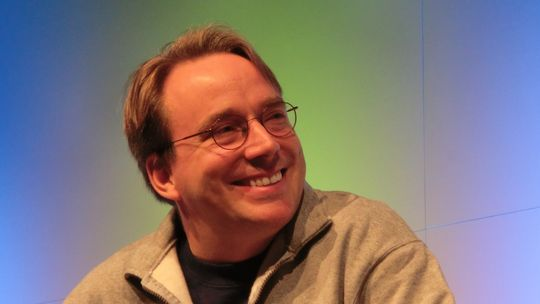
\includegraphics[width=50mm]{images/linus-torvalds.jpg}
	\caption{Linus Torvalds}
\end{figure}

La prima versione di \textbf{Linux} è la A e la B, fatta solamente da due finestre. Da emulatore di terminale com'era pensato in origine Linux d lì il è stato espanso fino a crearci un vero e proprio sistema operativo \textbf{Linux 0.0.1} con un kernel funzionante.

Già nel 1992 il sistema era diventato molto importante. Torvalds decide dunque di rendere il sistema \textbf{indipendente} da MINIX (ci fu anche una disputa con Tanenbaum). Cambiò dunque la licenza adottando la GPL, che considerava buona per il suo sistema operativo, a prescindere dal software GNU stesso. Nascono inoltre già le prime distribuzioni basate su linux, come ad esempio SUSE, MCC o la prima distribuzione commerciale: LGX. Queste distribuzioni rendevano decisamente più facile l'utilizzo di Linux (di per sè molto complesso).

Nel 1994 viene rilasciato \textbf{Linux 1.0} e fu lo stesso Torvalds a presentarlo in una conferenza tenutasi ad Helsinki. Già allora era un sistema utilizzabile.

Ancora nel 1993 erano nate le prime versioni commerciali: Bolzern, Flagship e \textbf{Linux Pro}. Nel 1994 nasce inoltre \textbf{RedHat}, creato da Marc Ewing, e diventa ben presto la più diffusa distribuzione Linux.

Nel 1996 fu scelto come logo ufficiale di Linux un pinguino disegnato da Larry Ewing, chiamato \textbf{Tux}, come abbreviazione di \textbf{T}orvalds \textbf{U}nix.

Sempre nel 1996 esce \textbf{Linux 2.0} con supporto a microprocessore. Con la versione 3.0, uscita nel 2011, le modifiche sono state molto più incrementali. Nel corso degli anni con la 2.0 il grado di utenza era ancora molto piccolo.

\begin{table}[htp]
	\centering
	\begin{tabular}[c]{l | l | l}
		\hline
		& 1992 & 2012 \\
		\hline
		Sviluppatori Linux & 100 & 1000 \\
		\hline
		Linee di codice Linux & 250.000 & 14.000.000 \\
		\hline
	\end{tabular}
	\caption{Sviluppo di Linux negli anni}
\end{table}

Una volta c'erano molti sviluppatori \textit{volontari}, ad oggi il supporto è dato da grosse aziende che possono investire tempo e denaro su Linux.

\subsection{Debian}

C'era un forte legame tra il mondo degli hackers e il mondo del software libero. Si venne a creare una \textbf{nuova generazione di sviluppatori}. Volevano provare a costruire una distribuzione che fosse fortemente legata a certi principi, che mettesse insieme varie cose, che facesse da collante. A quel punto nacque \textbf{Debian}. Linux da un lato stava procedendo e crescendo velocemente ed aveva molte caratteristiche interessanti, ma dall'altro c'era una lontananza dai principi del software libero e dalla GNU. Questo era percepito come un problema da parte di una fetta della comunità. Ad altri invece la cosa andava più che bene, dunque si venne a creare una \textbf{divergenza}. 

Il progetto Debian venne fondato da Ian Murdock nel 1993, con l'intento di fare una distribuzione di Linux \textbf{completamente libera}. Entrò a far parte del progetto GNU nel 1994-1995. Nel 1994 venne redatto il \textbf{manifesto debian}, nel quale si riassumeva il significato e la filosofia di Debian. La prima versione stabile (Debian 1.1 ``Buzz'') venne rilasciata nel 1996. Il project leader della Debian divenne Bruce Perens

La caratteristica principale di Debian è che pone l'attenzione in modo quasi maniacale alla qualità del software (a volte perdendo anche molto tempo) e al fatto che il software sia libero (solo software DFSG. Si basa su una \textbf{forte comunità} che gestisce (tramite votazioni) tutte le decisioni sullo sviluppo; chiunque può proporre cambiamenti e ognuno è responsabile delle proprie azioni (attenzione alla sicurezza). Un altro cardine su cui puntano gli sviluppatori Debian è una strenua \textbf{disponibilità} del software.

Debian è caratterizzato da un suddivisione (politica) in più parti del repository. Le uniche componenti che sono della Debian sono quelle libere e quelle che dipendono da software libero. Il software che è all'interno della Debian entra nell'archivio principale, \textbf{FREE}. Poi all'interno ci sono altre componenti ospitate nel server della Debian ma che non sono della Debian, \textbf{NON-FREE} che non aderisce alle \textit{DFSG}, \textbf{CONTRIB} (che è libero ma dipende da componenti non libere).

C'è una versione di Debian \textbf{stabile} (software un po' vecchio però), quella che ha superato tutti i bugfix, una versione \textbf{non stabile} e una versione \textbf{testing}. Nella versione non stabile ``\textit{può esplodere tutto da un momento all'altro}'', viene aggiornata ogni giorno. La testing entra nel pacchetto solamente se nell'ultimo mese non sono stati segnalati bug importanti.

Da un lato Debian ha molto software e dall'altro non avendo interessi commerciali, non ha interessi nel penalizzare la concorrenza. È gestita essenzialmente da volontari.

\subsection{Un po' di ordine}

\begin{itemize}
	\item Stallman con il progetto GNU voleva creare un nuovo sistema operativo, alternativo ad UNIX.
	\item Vengono sviluppati vari programmi, ma manca ancora un kernel. GNU Hurd doveva essere il kernel, ma lo sviluppo è stato lento.
	\item Linus crea Linux e viene utilizzato come kernel per GNU.
	\item Con il tempo Linux cambia ed inizia ad utilizzare anche del software proprietario. Diventano quindi distinti il progetto GNU e Linux. GNU/Linux è una distribuzione che utilizza una versione di Linux completamente libera. Al giorno d'oggi esistono anche GNU/Hurd e GNU/kFreeBSD.
	\item Linux è pubblicato sotto licenza GPLv2.
\end{itemize}
